\begin{table*}[h]\footnotesize
    \centering
    \caption{Contents and declaration methods of XML elements and attributes}
    \label{tab:xml-elements}
    
    \rowcolors{3}{lightgray}{}    

    \begin{threeparttable}    
        \begin{tabu} to \textwidth { X[4l] | X[0.8c] X[1.4c] X[1.5c] | X[8l] }
            \hline
            
                \multirow{2}{*}{\textbf{XML construct}}           &
                \multicolumn{3}{c|}{\textbf{Content}}      &
                \multirow{2}{*}{\textbf{Type declaration method}}     \\
                \cline{2-4}
                                        &   \textbf{Text}    &   \textbf{Elements}    &   \textbf{Attributes}      &                    \\
                                        
                                        
                % XML construct           &   Wrapped \newline Text    &   Wrapped \newline Elements    &   Attributes      &   Type declaration method     \\
                                        % &   Text    &   Elements    &   Attributes      &                    \\
            \hline
                Attribute                 &   Yes     &   No          &   No              &   \texttt{xs:simpleType}     \\            Simple element                 &   Yes     &   No          &   No              &   \texttt{xs:simpleType}                       \\
                Empty complex element           &   No      &   No          &   Yes             &   \texttt{xs:complexType} + [\texttt{xs:complexContent}] + attributes\tnotex{tnote:attribute-declarations} \\
                Text-only complex element      &   Yes     &   No          &   Yes             &   \texttt{xs:complexType} + \texttt{xs:simpleContent}  + attributes \\
                Element-only complex \newline element    &   No      &   Yes         &   Yes             &   \texttt{xs:complexType} + [\texttt{xs:complexContent}] \newline + elements\tnotex{tnote:element-declarations} + attributes \\
                Mixed complex element          &   Yes     &   Yes         &   Yes             &   \texttt{xs:complexType} + [\texttt{xs:complexContent}] \newline + \texttt{mixed} flag + elements + attributes \\
            \hline
        \end{tabu}
        \begin{tablenotes}
          \item\label{tnote:attribute-declarations} Attribute declarations
          \item\label{tnote:element-declarations} Element declarations
        \end{tablenotes}
    \end{threeparttable}    
\end{table*}

\subsubsection{XSD-based data models}\label{sec:xsd-based-data-models}

\paragraphx{\\XML elements, attributes and types}

An XSD-based data model may be described using one or more interrelated XSD schemas.
Each schema is a kept in a separate document and then the document can be imported by other XSD schemas and XML instance documents (XML datasets).
For instance, the CityGML data model consists of many XSD schemas, which address specific subdomains such as bridge, building, city furniture, land use, tunnel, etc.
These schemas import other base XSD schemas, such as GML and CityGMLBase.



An XML schema contains declarations of XML elements and their attributes.
XML elements can be either simple or complex.
\emph{Simple elements}, like attributes, may only have text content.
Whereas, \emph{complex elements} can wrap text and/or children elements, in addition to attributes, depending on whether they are
\emph{empty}, \emph{text-only}, \emph{element-only}, or \emph{mixed} complex elements (see \autoref{tab:xml-elements}).

There are two kinds of XSD types: simple and complex.
\emph{Simple types} are used for declaring simple elements and attributes, which only have text content.
\emph{Complex types} are applied only for complex elements.
Each type has a base type.
The top base type for simple types is \texttt{xs:anySimpleType}, and the top base type for all types is \texttt{xs:anyType}.

A simple type can be defined as (i) a \emph{list} of an existing simple type, or (ii) a \emph{union} of several existing simple types, or (iii) a copy of an existing simple type with some \emph{restrictions}.
XSD provides multiple kinds of restrictions for simple types:
\begin{itemize}
    \item \texttt{enumeration} defines a list of acceptable values.
    \item \texttt{length}, \texttt{min\-Length}, and \texttt{max\-Length} define a number of string characters or list items.
    \item \texttt{min\-Inclu\-sive}, \texttt{max\-Inclu\-sive}, \texttt{min\-Exclu\-sive}, and \texttt{max\-Exclu\-sive} define lower and upper bounds for numeric values.
    \item \texttt{pattern} defines a character pattern for string values.
    \item \texttt{totalDigits} and \texttt{fractionDigits} define numbers of digits in total and after the decimal point allowed in a number.
\end{itemize}

Complex types may have either \emph{simple content} or \emph{complex content}, both can include \emph{attribute declarations} such as attribute (\texttt{xs:attribute}), attribute group (\texttt{xs:attri\-bute\-Group}), and \emph{any}-attribute (\texttt{xs:anyAttribute}).
Any-attributes, like any-elements (see below), are attributes and elements undefined by the schema.
Each attribute may occur in an element not more than once, and can be declared as \emph{optional} (default) or \emph{required}.
Complex types with simple content are used for text-only complex element.
Complex types with complex content are needed for the rest kinds of complex elements.
The complex content may contain children \emph{element declarations} such as element (\texttt{xs:element}), element group (\texttt{xs:group}), or \emph{any}-element (\texttt{xs:any}).
Elements in a complex content must be defined with exact one of \emph{order indicators}:
(i) \texttt{sequence} allows child elements to occur in any order;
(ii) \texttt{all} allows child elements to occur in the order as defined;
and (iii) \texttt{choice} allows only one of the child elements to occur.
Regardless of which order indicator is used, elements can be specified with \texttt{min\-Occurs}, \texttt{max\-Occurs} and \texttt{nillable} attributes.
The complex content for mixed complex elements must be marked with \texttt{mixed} flag.


All elements and attributes have their own names, which are unique inside their parent element.
An element can be \emph{substituted} by another element with another name and type.
In contrast, XSD types can be \emph{anonymous}.
An anonymous XSD type can be used for its owner construct (an element or a parent type).
Besides, all elements, attributes, and types can have \emph{annotations}.

Elements and complex types may be declared as \emph{abstract}.
XML datasets can only contain non-abstract elements with non-abstract types.
In other words, abstract elements and types must be substitued and derived by others to be used in XML instance documents.



% Unique keys?



\bigskip\paragraphx{XSD-based building data formats}


Although the powerful XSD language allows describing almost any data model, building data formats, which are based on \emph{entity-based} conceptual models, utilise only certain element structures and types of XSD.
\autoref{tab:entity-models-to-xsd} shows a few common practices of how entity-based models are represented as XSD schemas, and how they could be parsed back from XSD schemas when needed.
The list of XSD-based data formats taken for the analysis are the followings: IFC-XML (ifcXML), COBieLite, CityGML, bsDD, and LandXML.

\begin{table}[h]\footnotesize
    \centering
    \caption{Contents and declaration methods of XML elements}
    \label{tab:data-model-to-xml}
    
    % \rowcolors{2}{}{lightgray}
    \begin{threeparttable}
        \begin{tabu} to \columnwidth { l X[l] }
            \hline
                \textbf{Model item}  &   \textbf{XML construct}         \\
            \hline
                \textbf{Instances}  &                      \\
                Entity              &   Empty, element-only, or mixed\tnotex{tn:mixed-element} complex element                      \\
                Entity explicit attribute    &   Attribute or Element-only complex element                      \\
                Entity derived attribute    &   Ignored (always)                      \\
                Entity inverse attribute    &   Ignored (with some exceptions)                     \\
            \hline
                \textbf{Types}      &                      \\
                Entity type         &   Complex type \newline with a sequence-list\tnotex{tn:choice-instead-sequence} of elements   \\
                Select type         &   Complex type \newline with a choice-list of elements \\
                Enumeration type    &   Simple type with an \texttt{enumeration} restriction \\
                Aggregation type    &   Simple type as \texttt{xs:list} of simple type or Complex type with a list\tnotex{tn:choice-instead-sequence} of elements \\
                Defined type        &   Similarly to its underlying type     \\
                Primitive type      &   Undeclared \\
            \hline
        \end{tabu}
        \begin{tablenotes}
          \item \label{tn:mixed-element} Mixed complex element is used rarely and mainly for addresses with mixed arbitrary and formatted texts.
          \item \label{tn:choice-instead-sequence} If there is only one element, either of order indicators \texttt{sequence}, \texttt{choice} or \texttt{all} can be used.          
        \end{tablenotes}
    \end{threeparttable}
\end{table}



% As can be seen in \autoref{tab:data-model-to-xml}, entities usually are mapped into empty or element-only complex XML element.
\autoref{lst:ifc-xsd-type-IfcAppliedValue} shows a fragment of the ifcXML4 XSD schema, mapped from an equivalent fragment of the IFC-EXPRESS schema  \autoref{lst:ifc-express-type-IfcAppliedValue}.
ENSPRESS entity type \texttt{IfcAppliedValue} is converted into (i) an element-only complex XML element for entity instances and (ii) a complex type.
% In this case both of them have the same name as the original entity type, however, usually type names have a "type" suffix.
% In IFC-XSD schema derived from IFC-EXPRESS, type names do not have the "type" suffix.
% Therefore, XML elements for entities and XML types for entity types have the same name.
This complex type has a complex content with a \texttt{sequence}-list of child elements, namely \texttt{AppliedValue}, \texttt{UnitBasis}, and \texttt{Components}.
Each of them stands for an entity type attribute with a select or an entity type.
Attribute \texttt{UnitBasis} also has type \texttt{IfcAppliedValue} as its parent type.
Select type \texttt{IfcAppliedValueSelect} of attribute \texttt{AppliedValue} is represented as a \texttt{choice}-group of complex elements, such as \texttt{IfcDate-wrapper} and \texttt{IfcMeasureWithUnit}.
The aggregation type of attribute \texttt{Components} is mapped to a complex type with the only element \texttt{IfcAppliedValue} having "unbounded" \texttt{maxOccurs} indicator.
This complex type also has attributes \texttt{itemType}, \texttt{cType}, and \texttt{arraySize}, which facilitate recognition of the aggregation item type, the aggregation kind, and the aggregation size.
In addition, complex type \texttt{IfcAppliedValue} has several attributes, which present entity type attributes with enumeration types or defined types, which are based on primitive types.
For instance, attribute \texttt{ArithmeticOperator} has an enumeration type \texttt{IfcArithmeticOperatorEnum}, represented as a simple type with an \texttt{enumeration} restriction.
Whereas, attributes \texttt{Name}, \texttt{Description}, and \texttt{ApplicableDate} have defined types \texttt{IfcLabel}, \texttt{IfcText}, and \texttt{IfcDate}, all of which are based on simple types \texttt{xs:normalizedString}.

% As mentioned, EXPRESS attributes, if they are converted into XML elements in IFC-XSD schema, then only to element-only complex elements.
% Similarly, select type 

% are always mapped either to XML attributes or element-only complex attributes.

% both EXPRESS types and attributes can be translated into XML elements. 

% \
% Inverse attributes are not mapped in the XSD schema.


% Both 



% <xs:element name="IfcCostValue" type="ifc:IfcCostValue" substitutionGroup="ifc:IfcAppliedValue" nillable="true"/>

% <xs:complexType name="IfcCostValue">
%   <xs:complexContent>
%     <xs:extension base="ifc:IfcAppliedValue"/>
%   </xs:complexContent>
% </xs:complexType>



\begin{lstlisting}[caption={ifcXML4 XSD schema: Element \texttt{IfcAppliedValue} and related types},label=lst:ifc-xsd-type-IfcAppliedValue]
  
<xs:element name="IfcAppliedValue" type="ifc:IfcAppliedValue" substitutionGroup="ifc:Entity" nillable="true"/>

<xs:complexType name="IfcAppliedValue">
  <xs:complexContent>
    <xs:extension base="ifc:Entity">
      <xs:sequence>
        <xs:element name="AppliedValue" nillable="true" minOccurs="0">
          <xs:complexType>
            <xs:group ref="ifc:IfcAppliedValueSelect"/>
          </xs:complexType>
        </xs:element>
        <xs:element name="UnitBasis" type="ifc:IfcMeasureWithUnit" nillable="true" minOccurs="0"/>
        <xs:element name="Components" nillable="true" minOccurs="0">
          <xs:complexType>
            <xs:sequence>
              <xs:element ref="ifc:IfcAppliedValue" maxOccurs="unbounded"/>
            </xs:sequence>
            <xs:attribute ref="ifc:itemType" fixed="ifc:IfcAppliedValue"/>
            <xs:attribute ref="ifc:cType" fixed="list"/>
            <xs:attribute ref="ifc:arraySize" use="optional"/>
          </xs:complexType>
        </xs:element>
      </xs:sequence>
      <xs:attribute name="Name" type="ifc:IfcLabel" use="optional"/>
      <xs:attribute name="Description" type="ifc:IfcText" use="optional"/>
      <xs:attribute name="ApplicableDate" type="ifc:IfcDate" use="optional"/>
      ...
      <xs:attribute name="ArithmeticOperator" type="ifc:IfcArithmeticOperatorEnum" use="optional"/>
    </xs:extension>
  </xs:complexContent>
</xs:complexType>
</xs:element>

<xs:group name="IfcAppliedValueSelect">
  <xs:choice>
    ...
    <xs:element ref="ifc:IfcAreaMeasure-wrapper"/>
    <xs:element ref="ifc:IfcDate-wrapper"/>
    <xs:element ref="ifc:IfcMeasureWithUnit"/>
    ...
  </xs:choice>
</xs:group>

<xs:element name="IfcDate-wrapper" nillable="true">
  <xs:complexType>
    <xs:simpleContent>
      <xs:extension base="ifc:IfcDate">
        <xs:attributeGroup ref="ifc:instanceAttributes"/>
      </xs:extension>
    </xs:simpleContent>
  </xs:complexType>
</xs:element>

<xs:simpleType name="IfcDate">
  <xs:restriction base="xs:normalizedString"/>
</xs:simpleType>

<xs:element name="IfcMeasureWithUnit" type="ifc:IfcMeasureWithUnit" ... />

<xs:complexType name="IfcMeasureWithUnit">
  <xs:complexContent>
    <xs:extension base="ifc:Entity">
      <xs:sequence>
        <xs:element name="ValueComponent">
          <xs:complexType>
            <xs:group ref="ifc:IfcValue"/>
          </xs:complexType>
        </xs:element>
        <xs:element name="UnitComponent">
          <xs:complexType>
            <xs:group ref="ifc:IfcUnit"/>
          </xs:complexType>
        </xs:element>
      </xs:sequence>
    </xs:extension>
  </xs:complexContent>
</xs:complexType>
  
<xs:simpleType name="IfcArithmeticOperatorEnum">
  <xs:restriction base="xs:string">
    <xs:enumeration value="add"/>
    <xs:enumeration value="divide"/>
    ...
  </xs:restriction>
</xs:simpleType>
\end{lstlisting}


% ENTITY IfcCostValue
%  SUBTYPE OF (IfcAppliedValue);
% END_ENTITY;

\begin{lstlisting}[caption={EXPRESS schema: entity type \texttt{IfcAppliedValue}},label=lst:ifc-xsd-entity-type]
ENTITY IfcAppliedValue
 SUPERTYPE OF (ONEOF (IfcCostValue));
  Name : OPTIONAL IfcLabel;
  Description : OPTIONAL IfcText;
  AppliedValue : OPTIONAL IfcAppliedValueSelect;
  UnitBasis : OPTIONAL IfcMeasureWithUnit;
  ApplicableDate : OPTIONAL IfcDate;
  FixedUntilDate : OPTIONAL IfcDate;
  Category : OPTIONAL IfcLabel;
  Condition : OPTIONAL IfcLabel;
  ArithmeticOperator : OPTIONAL IfcArithmeticOperatorEnum;
  Components : OPTIONAL LIST [1:?] OF IfcAppliedValue;
 INVERSE
  HasExternalReference : SET [0:?] OF IfcExternalReferenceRelationship FOR RelatedResourceObjects;
END_ENTITY;

TYPE IfcAppliedValueSelect = SELECT
  (IfcMeasureWithUnit, IfcReference, IfcValue);
END_TYPE;

ENTITY IfcMeasureWithUnit;
  ValueComponent : IfcValue;
  UnitComponent : IfcUnit;
END_ENTITY;




\end{lstlisting}




Although the gerenal 
Data structure almost the same.
Naming style are different.



Assume that we have an entity-based conceptual model.
Then its entity types can be mapped into either complex empty, or complex element-only, or complex mixed elements.
Entity attributes are represented as XML attributes, if their types can be mapped into XML simple types.
Otherwise, entity attributes are represented as XML elements wrapped in the parent complex element.
Wrapped elements of Complex Element-only or Complex Mixed elements are usually specified with order indicator \texttt{xs:sequence}.
However, if there is only one internal element, order indicator \texttt{xs:choice} also can be used.
In contrast, order indicator \texttt{xs:any} must be avoided.
Complex Mixed elements are used very rarely and mainly for addresses types (see \autoref{lst:xsd-entity-type-mixed-element}).

\begin{lstlisting}[caption={a},label=lst:xsd-entity-type-mixed-element]
<xs:element name="PostBoxNumberPrefix" minOccurs="0">
  <xs:annotation>
    <xs:documentation>Specification of the prefix of the post box number. eg. A in POBox:A-123</xs:documentation>
  </xs:annotation>
  <xs:complexType mixed="true">
    <xs:attribute name="NumberPrefixSeparator">
      <xs:annotation>
        <xs:documentation>A-12 where 12 is number and A is prefix and "-" is the separator</xs:documentation>
      </xs:annotation>
    </xs:attribute>
    <xs:attributeGroup ref="grPostal"/>
    <xs:anyAttribute namespace="##other"/>
  </xs:complexType>
</xs:element>
\begin{lstlisting}




Consider a typical example in \autoref{lst:xsd-entity-type}.
Element \texttt{IfcAppliedValue} is equivalent to entity type with the same name.
It has attributes \texttt{AppliedValue}, \texttt{UnitBasis}, and \texttt{Components}, which are represented as XML elements located in a strict order because order indicator \texttt{xs:sequence} is used.
On ther other hand, it has attributes represented as XML attributes such as \texttt{Name}, \texttt{Description}, etc.
Attribute \texttt{AppliedValue} has a select type \texttt{IfcAppliedValueSelect}.



(see \autoref{lst:xsd-entity-types}).





% <xs:element name="IfcWorkControl" type="ifc:IfcWorkControl" abstract="true" substitutionGroup="ifc:IfcControl" nillable="true"/>
% 	<xs:complexType name="IfcWorkControl" abstract="true">
% 		<xs:complexContent>
% 			<xs:extension base="ifc:IfcControl">
% 				<xs:sequence>
% 					<xs:element name="Creators" nillable="true" minOccurs="0">
% 						<xs:complexType>
% 							<xs:sequence>
% 								<xs:element ref="ifc:IfcPerson" maxOccurs="unbounded"/>
% 							</xs:sequence>
% 							<xs:attribute ref="ifc:itemType" fixed="ifc:IfcPerson"/>
% 							<xs:attribute ref="ifc:cType" fixed="set"/>
% 							<xs:attribute ref="ifc:arraySize" use="optional"/>
% 						</xs:complexType>
% 					</xs:element>
% 				</xs:sequence>
% 				<xs:attribute name="CreationDate" type="ifc:IfcDateTime" use="optional"/>
% 				<xs:attribute name="Purpose" type="ifc:IfcLabel" use="optional"/>
% 				<xs:attribute name="Duration" type="ifc:IfcDuration" use="optional"/>
% 				<xs:attribute name="TotalFloat" type="ifc:IfcDuration" use="optional"/>
% 				<xs:attribute name="StartTime" type="ifc:IfcDateTime" use="optional"/>
% 				<xs:attribute name="FinishTime" type="ifc:IfcDateTime" use="optional"/>
% 			</xs:extension>
% 		</xs:complexContent>
% 	</xs:complexType>
% 	<xs:element name="IfcWorkPlan" type="ifc:IfcWorkPlan" substitutionGroup="ifc:IfcWorkControl" nillable="true"/>
% 	<xs:complexType name="IfcWorkPlan">
% 		<xs:complexContent>
% 			<xs:extension base="ifc:IfcWorkControl">
% 				<xs:attribute name="PredefinedType" type="ifc:IfcWorkPlanTypeEnum" use="optional"/>
% 			</xs:extension>
% 		</xs:complexContent>
% 	</xs:complexType>





% \begin{lstlisting}[caption={A},label=lst:express-guid]
% <xs:complexType name="AbstractCityObjectType" abstract="true">
%  <xs:complexContent>
%   <xs:extension base="gml:AbstractFeatureType">
%      <xs:sequence>
%       <xs:element name="creationDate" type="xs:date" minOccurs="0"/>
%       <xs:element name="terminationDate" type="xs:date" minOccurs="0"/>
%       <xs:element name="externalReference" type="ExternalReferenceType" minOccurs="0" maxOccurs="unbounded"/>
%       <xs:element name="generalizesTo" type="GeneralizationRelationType" minOccurs="0" maxOccurs="unbounded"/>
%       <xs:element name="relativeToTerrain" type="RelativeToTerrainType" minOccurs="0"/>
%       <xs:element name="relativeToWater" type="RelativeToWaterType" minOccurs="0"/>
%       <xs:element ref="_GenericApplicationPropertyOfCityObject" minOccurs="0" maxOccurs="unbounded"/>
%      </xs:sequence>
%   </xs:extension>
%  </xs:complexContent>
% </xs:complexType>
% \end{lstlisting}












The survey shows that only several XSD types are often used in real building data formats.
The diagram in \autoref{fig:xsd-type-hierarchy} shows a fragment of the XSD type hierarchy, which includes all types met in the experiment and a few other types related to them.
Cyan boxes with bold borders, yellow boxes, and white boxes are respectively denote often, rarely, and never used types.
The most often used simple types, in descending order of use frequency, are the following:
\begin{itemize}
    \item \texttt{string} (Unicode string);
    \item \texttt{double} (64-bit floating point number);
    \item \texttt{normalizedString} (like \texttt{string}, but certain characters must be escaped, e.g. \texttt{\&lt;});
    \item \texttt{any} (top XSD type, mainly used for declaration of abstract elements);
    \item \texttt{long} (64-bit integer);
    \item \texttt{boolean};
    \item \texttt{integer} (arbitrary integer);
    \item \texttt{date};
    \item and \texttt{dateTime}.
\end{itemize}
Other numeric and binary types, for instance, \texttt{decimal} (decimal number of arbitrary precision and super type of all integer types), \texttt{int} (32-bit integer), \texttt{nonNegativeInteger}, and \texttt{hexBinary} are seldom used.
Other specific types can be met only 1-2 times, mainly in the ifcXML4\_Add2 schema.


\begin{figure}
    \centering    
    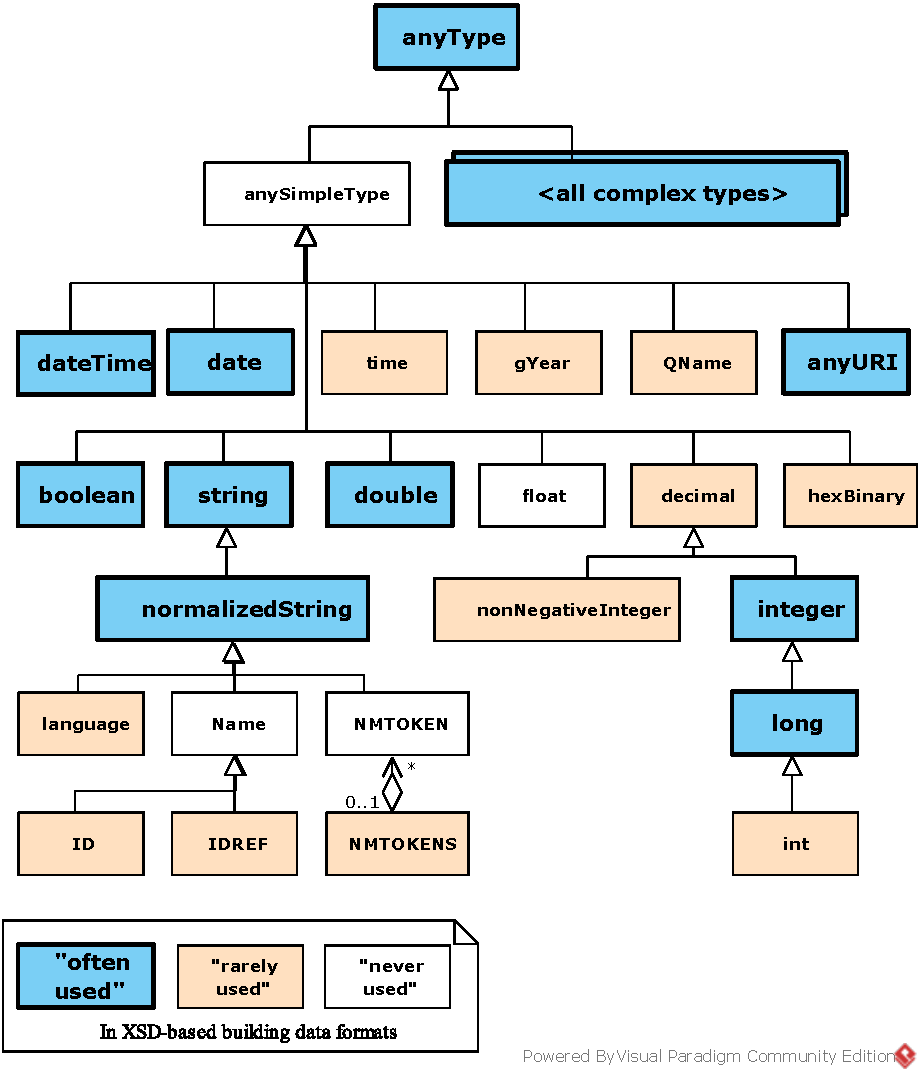
\includegraphics[width=\columnwidth]{images/xsd-type-hierarchy-8.pdf}
    % \caption{XSD type hierarchy\\\hspace{\textwidth}cyan, bold-border boxes}
     \caption{XSD types used in building data formats}
        % {\tabular[t]{@{}l@{}}XSD type hierarchy \\ This is the second line\endtabular}
    \label{fig:xsd-type-hierarchy}
\end{figure}




Simple type restriction \texttt{enumeration} is very often utilised in building data models for declaring enumeration types.
All 




